\section{Technical assessment of water hammer for expansion loops}
\subsection{Frequency of the water hammer pressure fluctuation in a pipe}
\subsubsection{Pressure fluctuation and associated frequencies analysis}
The maximum magnitude of the water hammer pulse is \eqref{jk1}. This is also known as the Joukowsky equation.
\begin{gather}\label{jk1}
    \Delta p = \rho a_0 \Delta v\, (\si{\pascal})
\end{gather}
where $\Delta p$ is the change in pressure, $\rho$ is the fluid density, $a_0$ is the sonic velocity in the pipe and $\Delta v$ is the change in fluid velocity. The sonic velocity can be determined through \eqref{sonic1}
\begin{gather}\label{sonic1}
    \frac{1}{a^2} = \frac{1}{c^2} + \frac{\rho D }{\tau E}
\end{gather}
where $c$ is the speed of sound in the fluid, $\rho$ is fluid density, $D$ is pipe internal diameter, $\tau$ is wall thickness of pipe and $E$ is Young's Modulus of pipe. Running the MATLAB script with the values shown in Table \ref{matlabScriptVals}, Figure \ref{pressure1} was generated.
\begin{table}[H]
    \centering
    \begin{tabular}{@{}ll@{}}
        \toprule
        \textbf{Parameter} & \textbf{Value}\\
        \midrule
        $c$ & \SI{1100}{\meter\per\second}\\
        $\rho$ & \SI{455}{\kilo\gram\per\meter\cubed}\\
        $D$ & \SI{793.94}{\milli\meter}\\
        $\tau$ & \SI{19.06}{\milli\meter}\\
        $E$ & \SI{200}{\giga\pascal}\\
        $\Delta v$ & \SI{1.5}{\meter\per\second}\\
        $a_0$ & \SI{1041.89}{\meter\per\second}\\
        \bottomrule
    \end{tabular}
    \caption{Values for Joukowski Prediction.}
    \label{matlabScriptVals}
\end{table}
\begin{figure}[H]
    \centering
    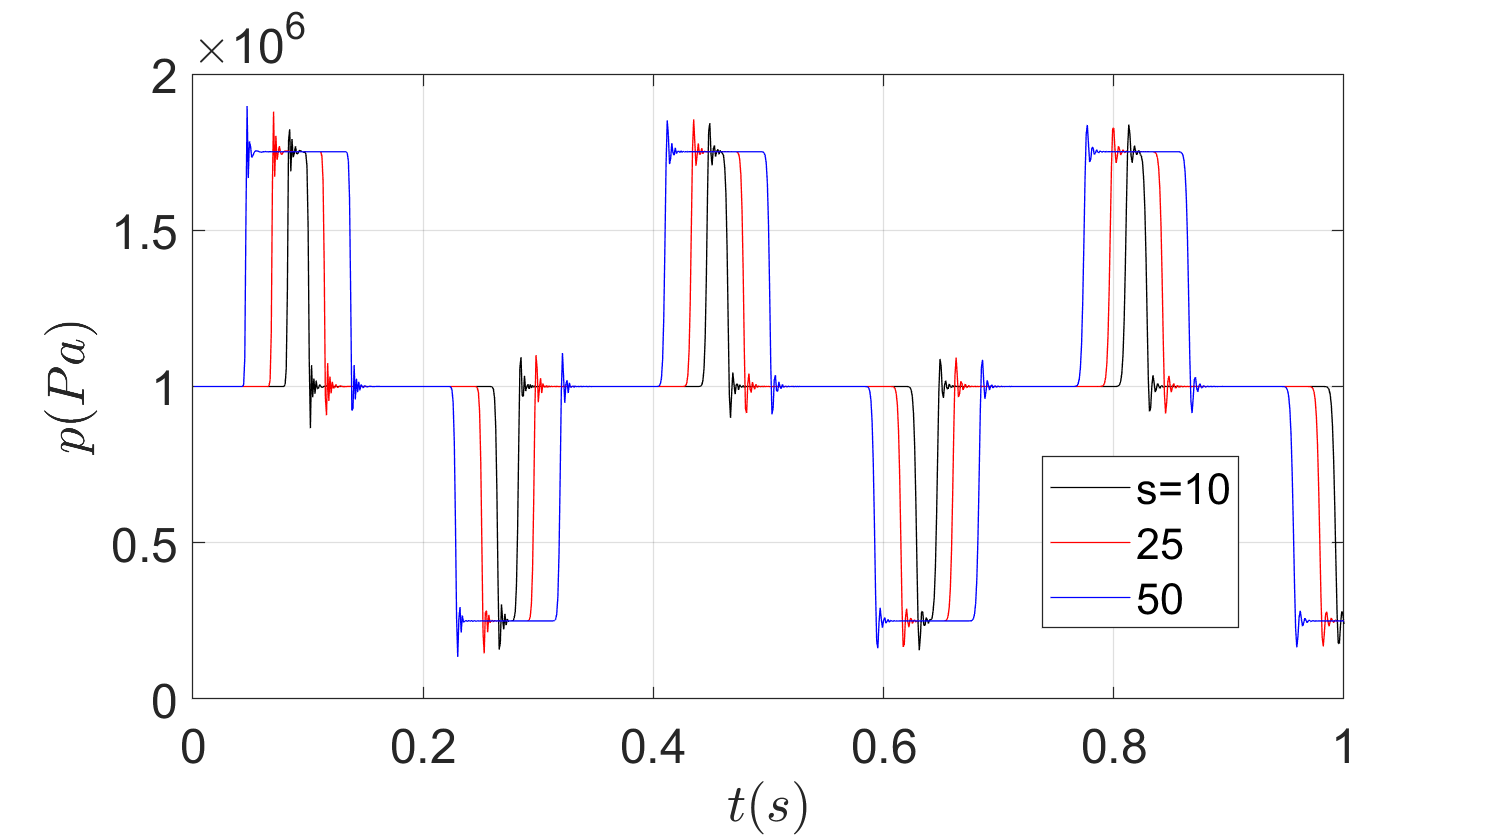
\includegraphics[width = 0.9 \textwidth]{img/fig1.png}
    \caption{MATLAB script results showing pressure against time for $s=10,\,25,\,\SI{50}{\meter}$.}
    \label{pressure1}
\end{figure}
\begin{figure}[H]
    \centering
    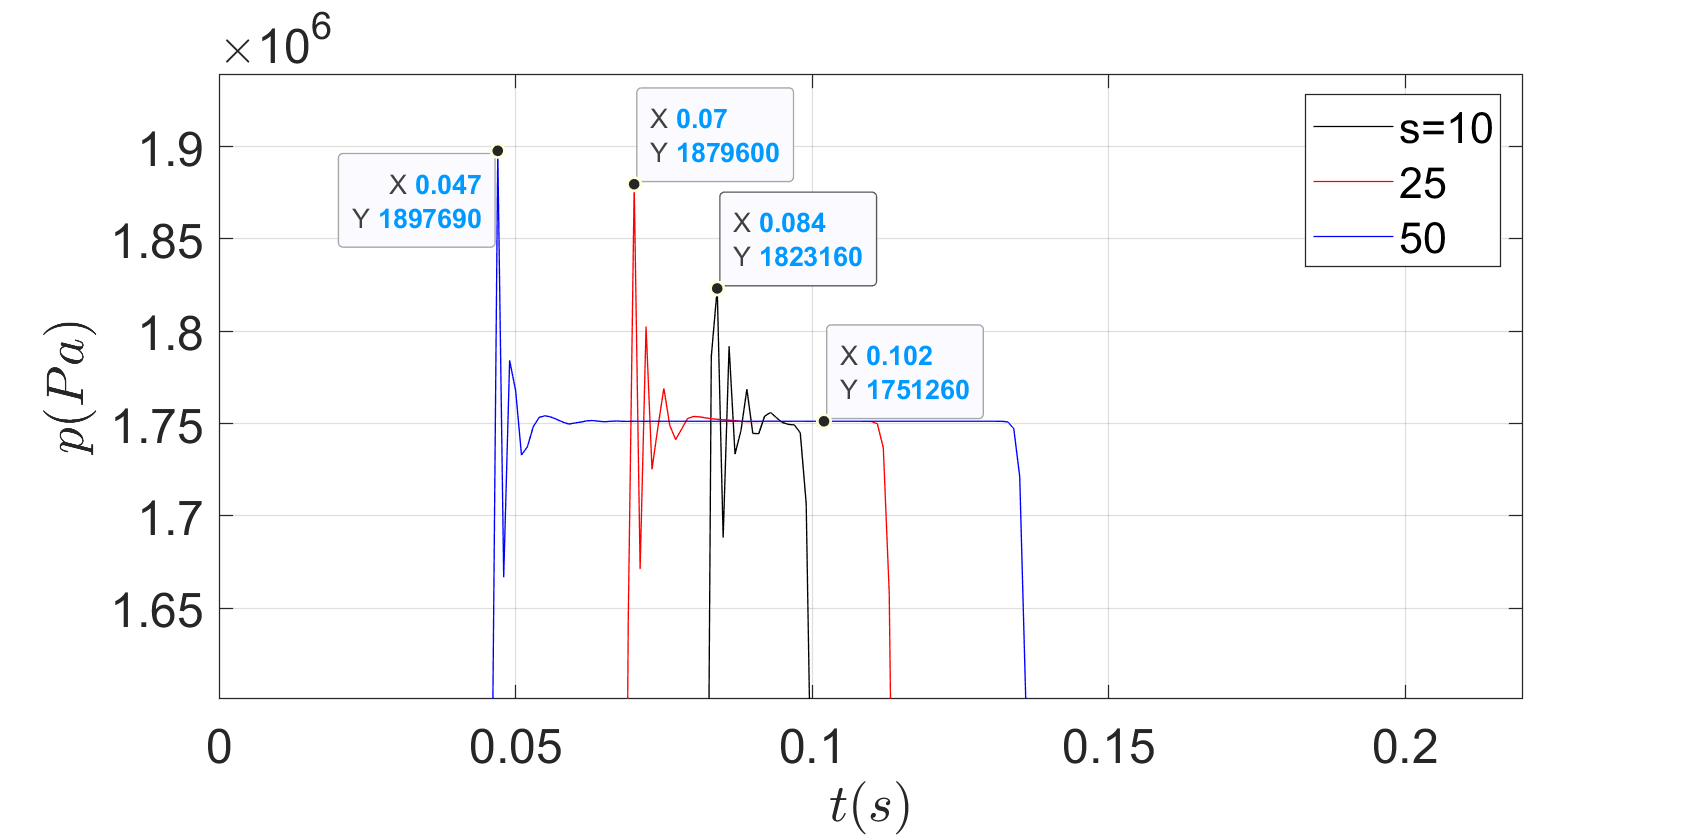
\includegraphics[width = 0.9 \textwidth]{img/fig3.png}
    \caption{Index points for finding maximum pressure differential and settled pressure differential.}
    \label{pressure2}
\end{figure}
Using the Joukowsky equation, we attain a value for our pressure differential:
\begin{gather}
    \Delta p_{joukowsky} = \SI{711087}{\pascal}
\end{gather}
Table \ref{matlabResults} shows the maximum pressure differentials for each index point ($s$- value) and the pressure differential of the settled value.
\begin{table}[H]
    \centering
    \begin{tabular}{@{}lll@{}}
        \toprule
        \textbf{$s$- value} & \textbf{Maximum pressure } & \textbf{Percentage difference}\\
        & \textbf{differential}/\si{\pascal} & \textbf{compared to analytical}\\
        \midrule
        10 & 823160 & 15.76\%\\
        25 & 879600 & 23.70\%\\
        50 & 897690 & 26.24\%\\
        Settled value & 751260 & 5.64\%\\
        \bottomrule
    \end{tabular}
    \caption{Pressure differentials for indexed $s$- values and settled values.}
    \label{matlabResults}
\end{table}
An analytical result for the frequencies of the pressure fluctuation can be found using \eqref{freq1}.
\begin{gather}\label{freq1}
    T = \frac{1}{f} = \frac{2L}{c} = \frac{2\cdot s}{1100}
\end{gather}
Analysing the period of the pressure differentials, we can  find that the frequencies of the pressure fluctuation in Table \ref{freq2}. The index points to find the periods of oscillation were selected as the first peak of the overshoot.
\begin{table}[H]
    \centering
    \begin{tabular}{@{}llll@{}}
        \toprule
        \textbf{$s$- value} & \textbf{Frequency}/\si{\hertz} & \textbf{Frequency}/\si{\hertz} & \textbf{Percentage}\\
        & \textbf{(MATLAB)} & \textbf{(Analytical)} & \textbf{difference}\\
        \midrule
        10 & 10.99 & 11 & 0.09\%\\
        25 & 21.74 & 22 & 1.18\%\\
        50 & 55.56 & 55 & 1.02\%\\
        \bottomrule
    \end{tabular}
    \caption{Frequency of pressure fluctuation.}
    \label{freq2}
\end{table}
\subsubsection{Forces acting on bend and direction of total force on expansion loop}
\subsection{Model analysis of expansion loop}
\subsection{Discussion and context}